\section{Introduction}
    \label{sec:intro}

    %* show the problem
    %* introduce the idea
    %* contributions?

    % introduce the problem
    Current state-of-the-art object recognition systems make predictions based on static images. These systems prove limited in cases when objects are in featureless or ambiguous orientations. An appropriate solution is to interact with the object and adjust its pose to reveal discriminative features for determining its identity.

    There are three canonical object recognition problems which highlight the need for interactive object recognition.

    1) Many real settings are littered with systematic bias. For object recognition, the most notorious are shadow and glare. Reorienting the object in such as way to reduce these biases would allow for more accurate object predictions.

    2) Many objects are ambiguous with other objects in certain poses. The back of a book may not be enough information to confidently determine what specific book is being observed. Flipping the book over and observing the cover would result in a more confident prediction. 

    3) Some objects may be so ambiguous that no single observation can confidently determine the identity of the object. Take for example, two identical featureless balls where one has a small mark on it. If a ball is observed only once with no mark on it, a static object recognition system could never be sure which ball it is observing because the mark could be obscured by the orientation. To resolve which ball is being observed, a robot must rotate the ball through all orientations remembering its previous observations before concluding that the mark is absent or not.

    This paper introduces a probabilistic graphical model for object and pose recognition that is agnostic of the types of  features used. This model is used to infer a distribution of posterior object probabilities conditioned on all previous actions and observations. An optimal actions is selected based on the criteria of improving the confidence of object predictions after the action is taken. To the best of our knowledge, we are the first to introduce the idea of a robot interacting with its environment to improve object recognition. 

    In this paper, we show that such a system works in determining the optimal actions to solve the ambiguous book problem shown in \figref{fig:pr2}

    \setlength{\tabcolsep}{0.1em}
    \begin{figure}[ht]
    \centering
    \begin{tabular}{cccc}
    \multicolumn{2}{c}{\multirow{-9}{*}{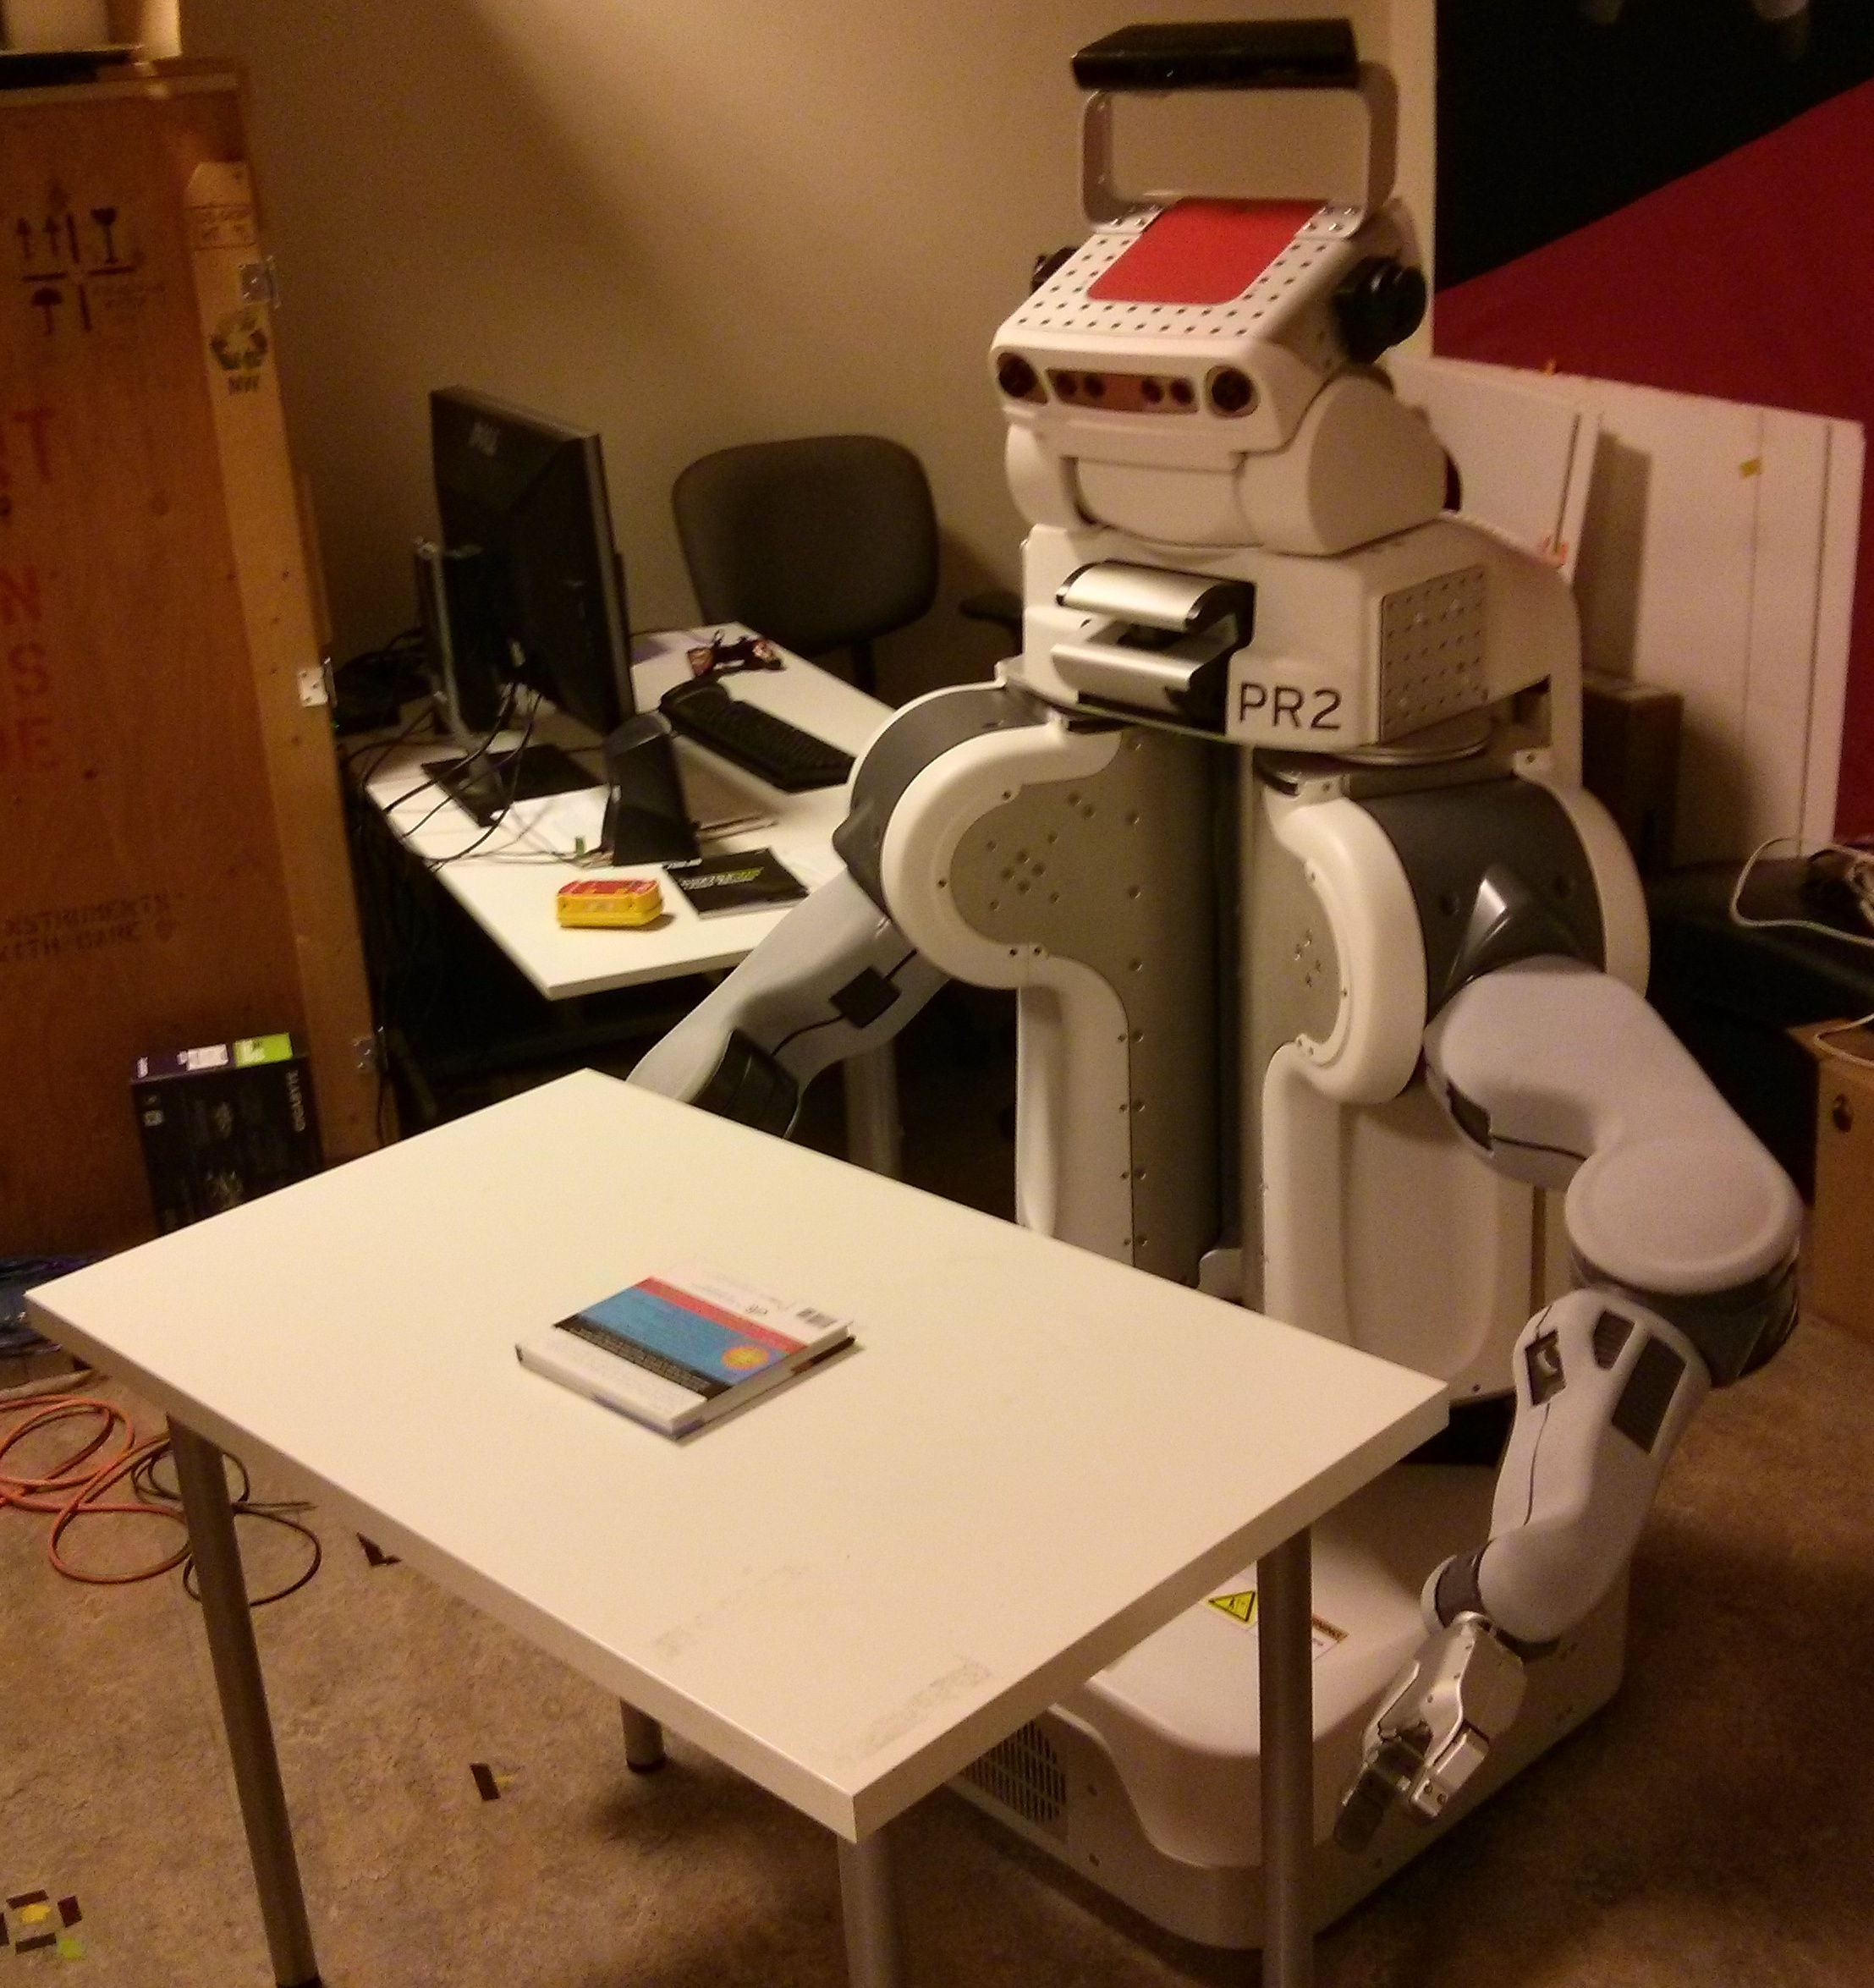
\includegraphics[width=0.46\columnwidth]{pics/pr2_init.jpg}}} & 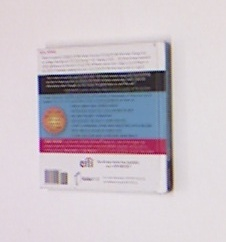
\includegraphics[width=0.23\columnwidth]{pics/first_back.jpg} 
    &
\includegraphics[width=0.23\columnwidth]{pics/first_cover1.jpg} \\
    \multicolumn{2}{c}{} & 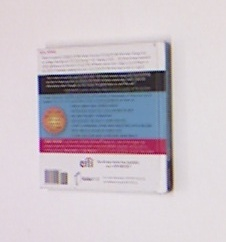
\includegraphics[width=0.23\columnwidth]{pics/first_back.jpg} 
    &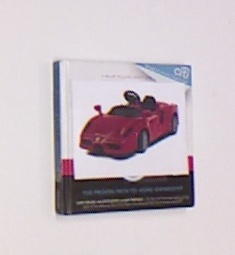
\includegraphics[width=0.23\columnwidth]{pics/first_cover2.jpg} \\
    \multicolumn{2}{c}{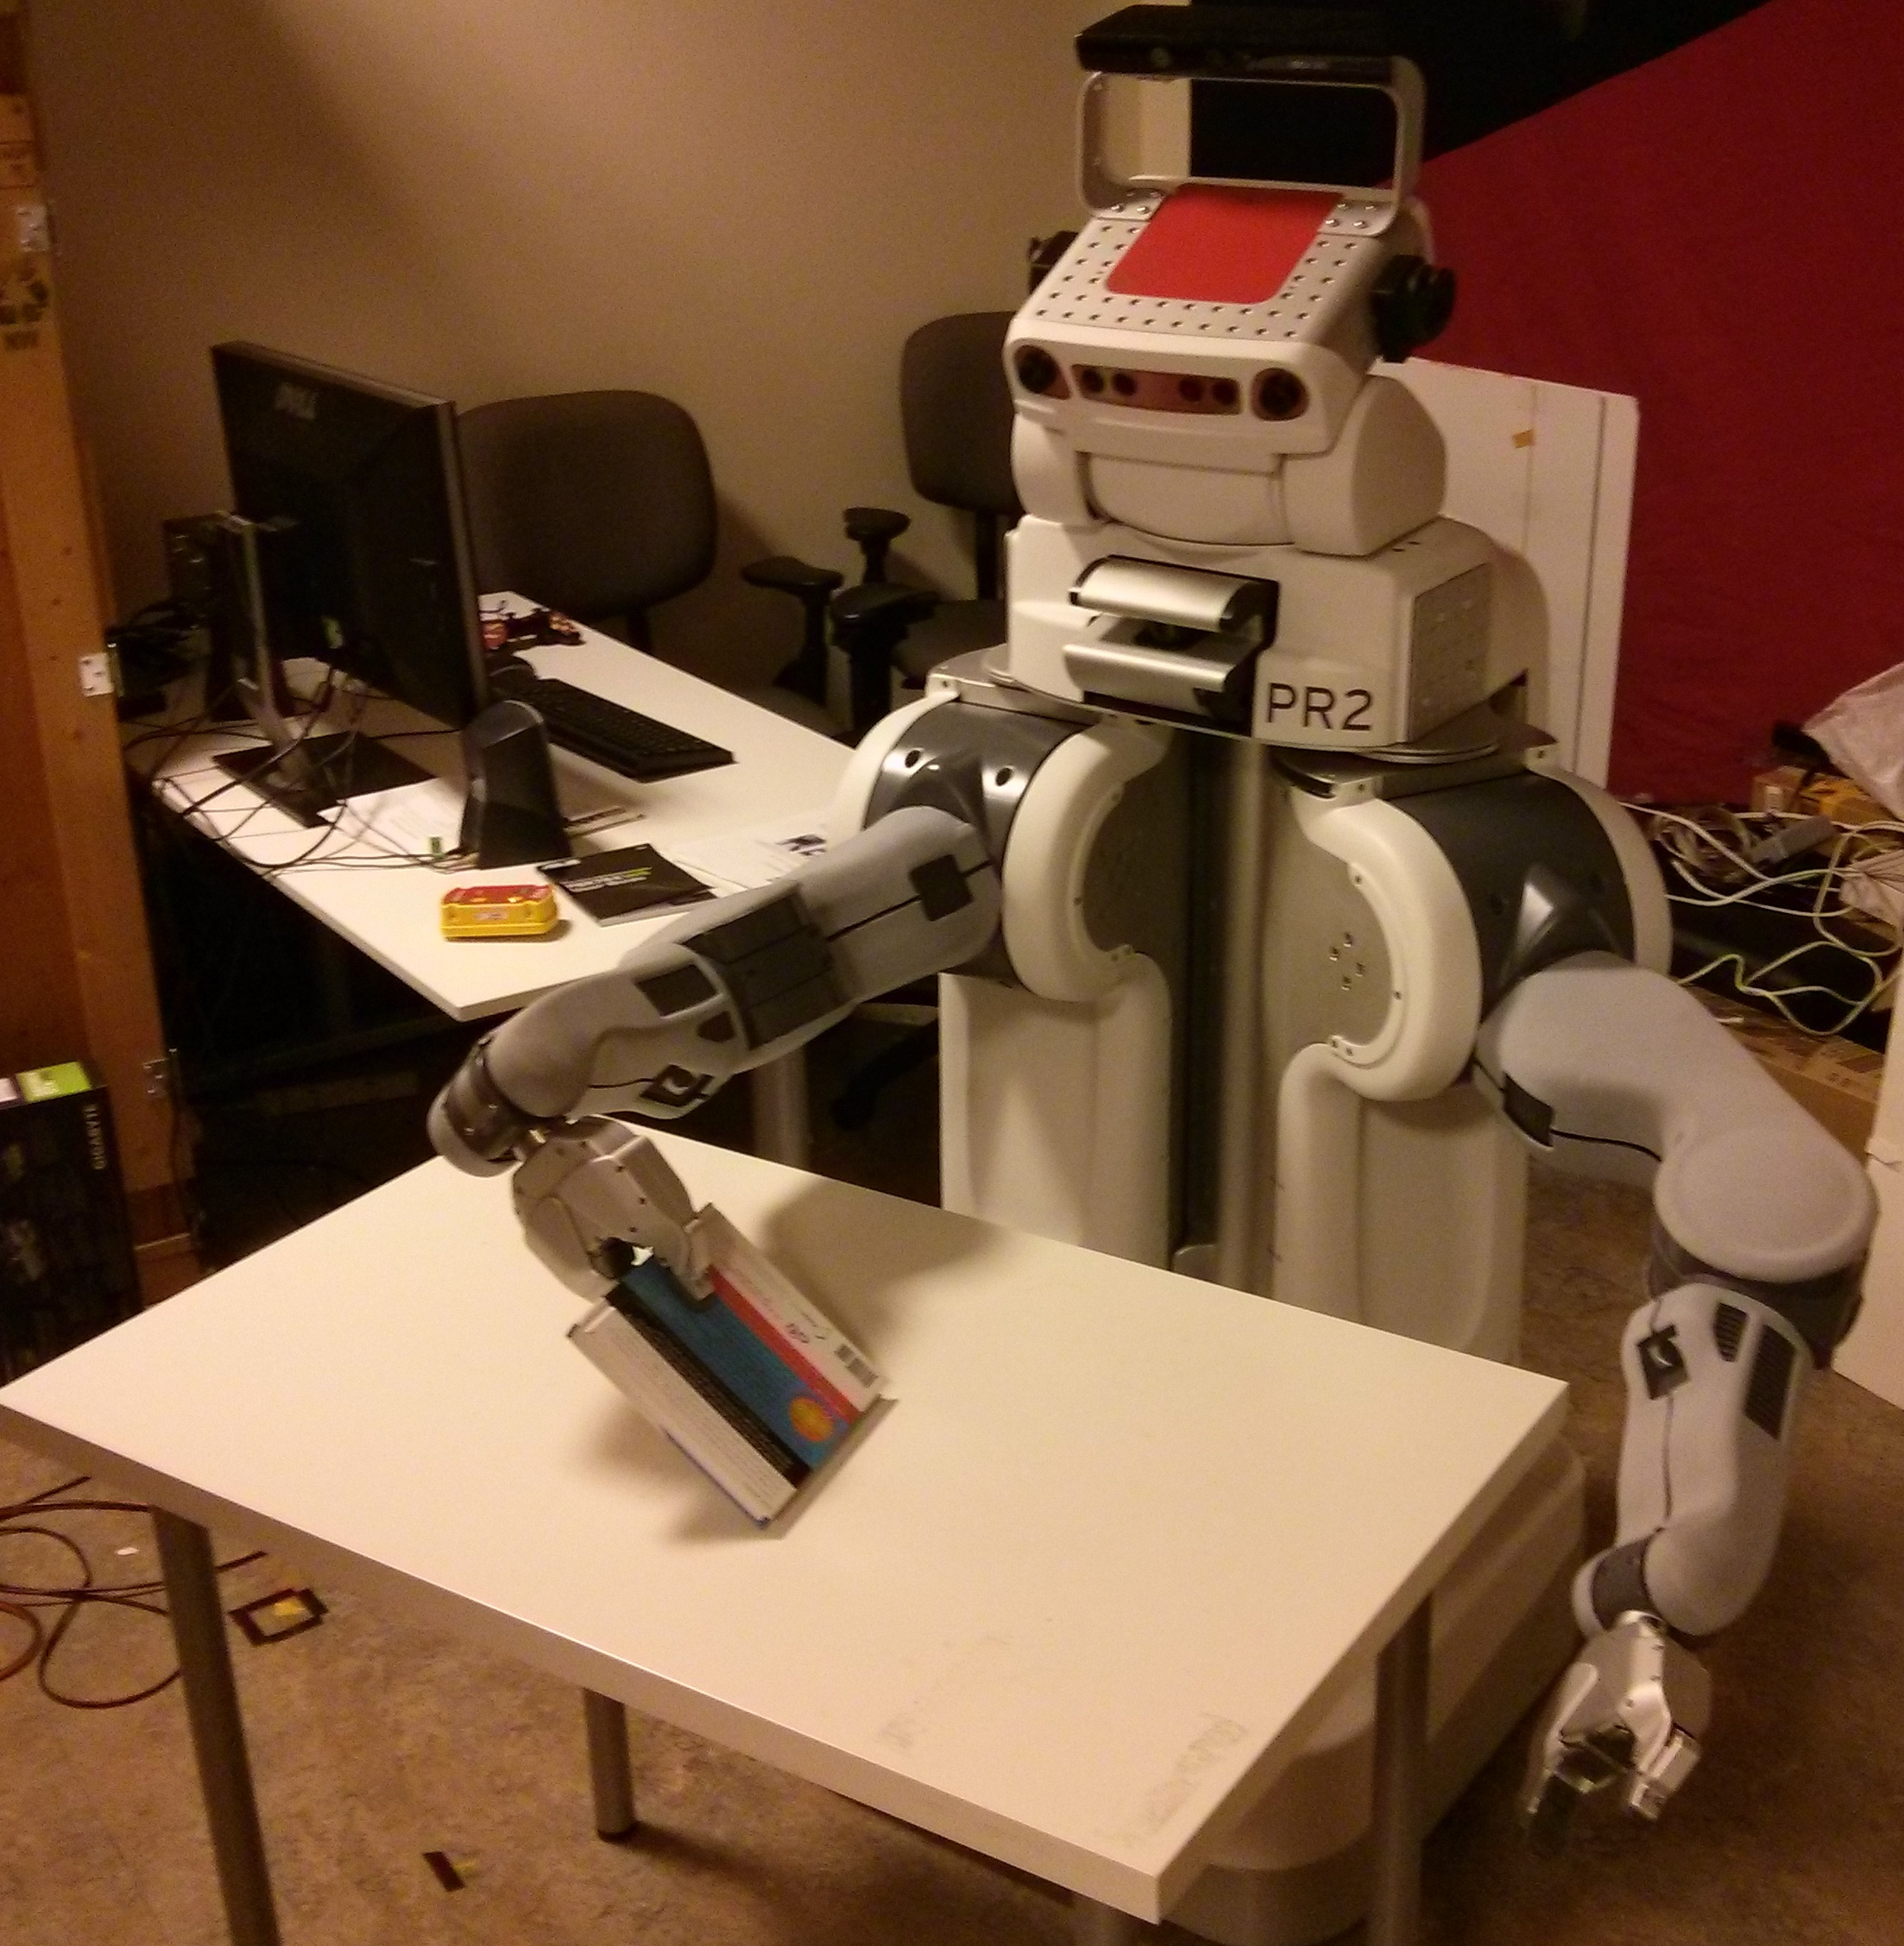
\includegraphics[width=0.45\columnwidth]{pics/pr2_grasp.jpg}}
    & \multicolumn{2}{c}{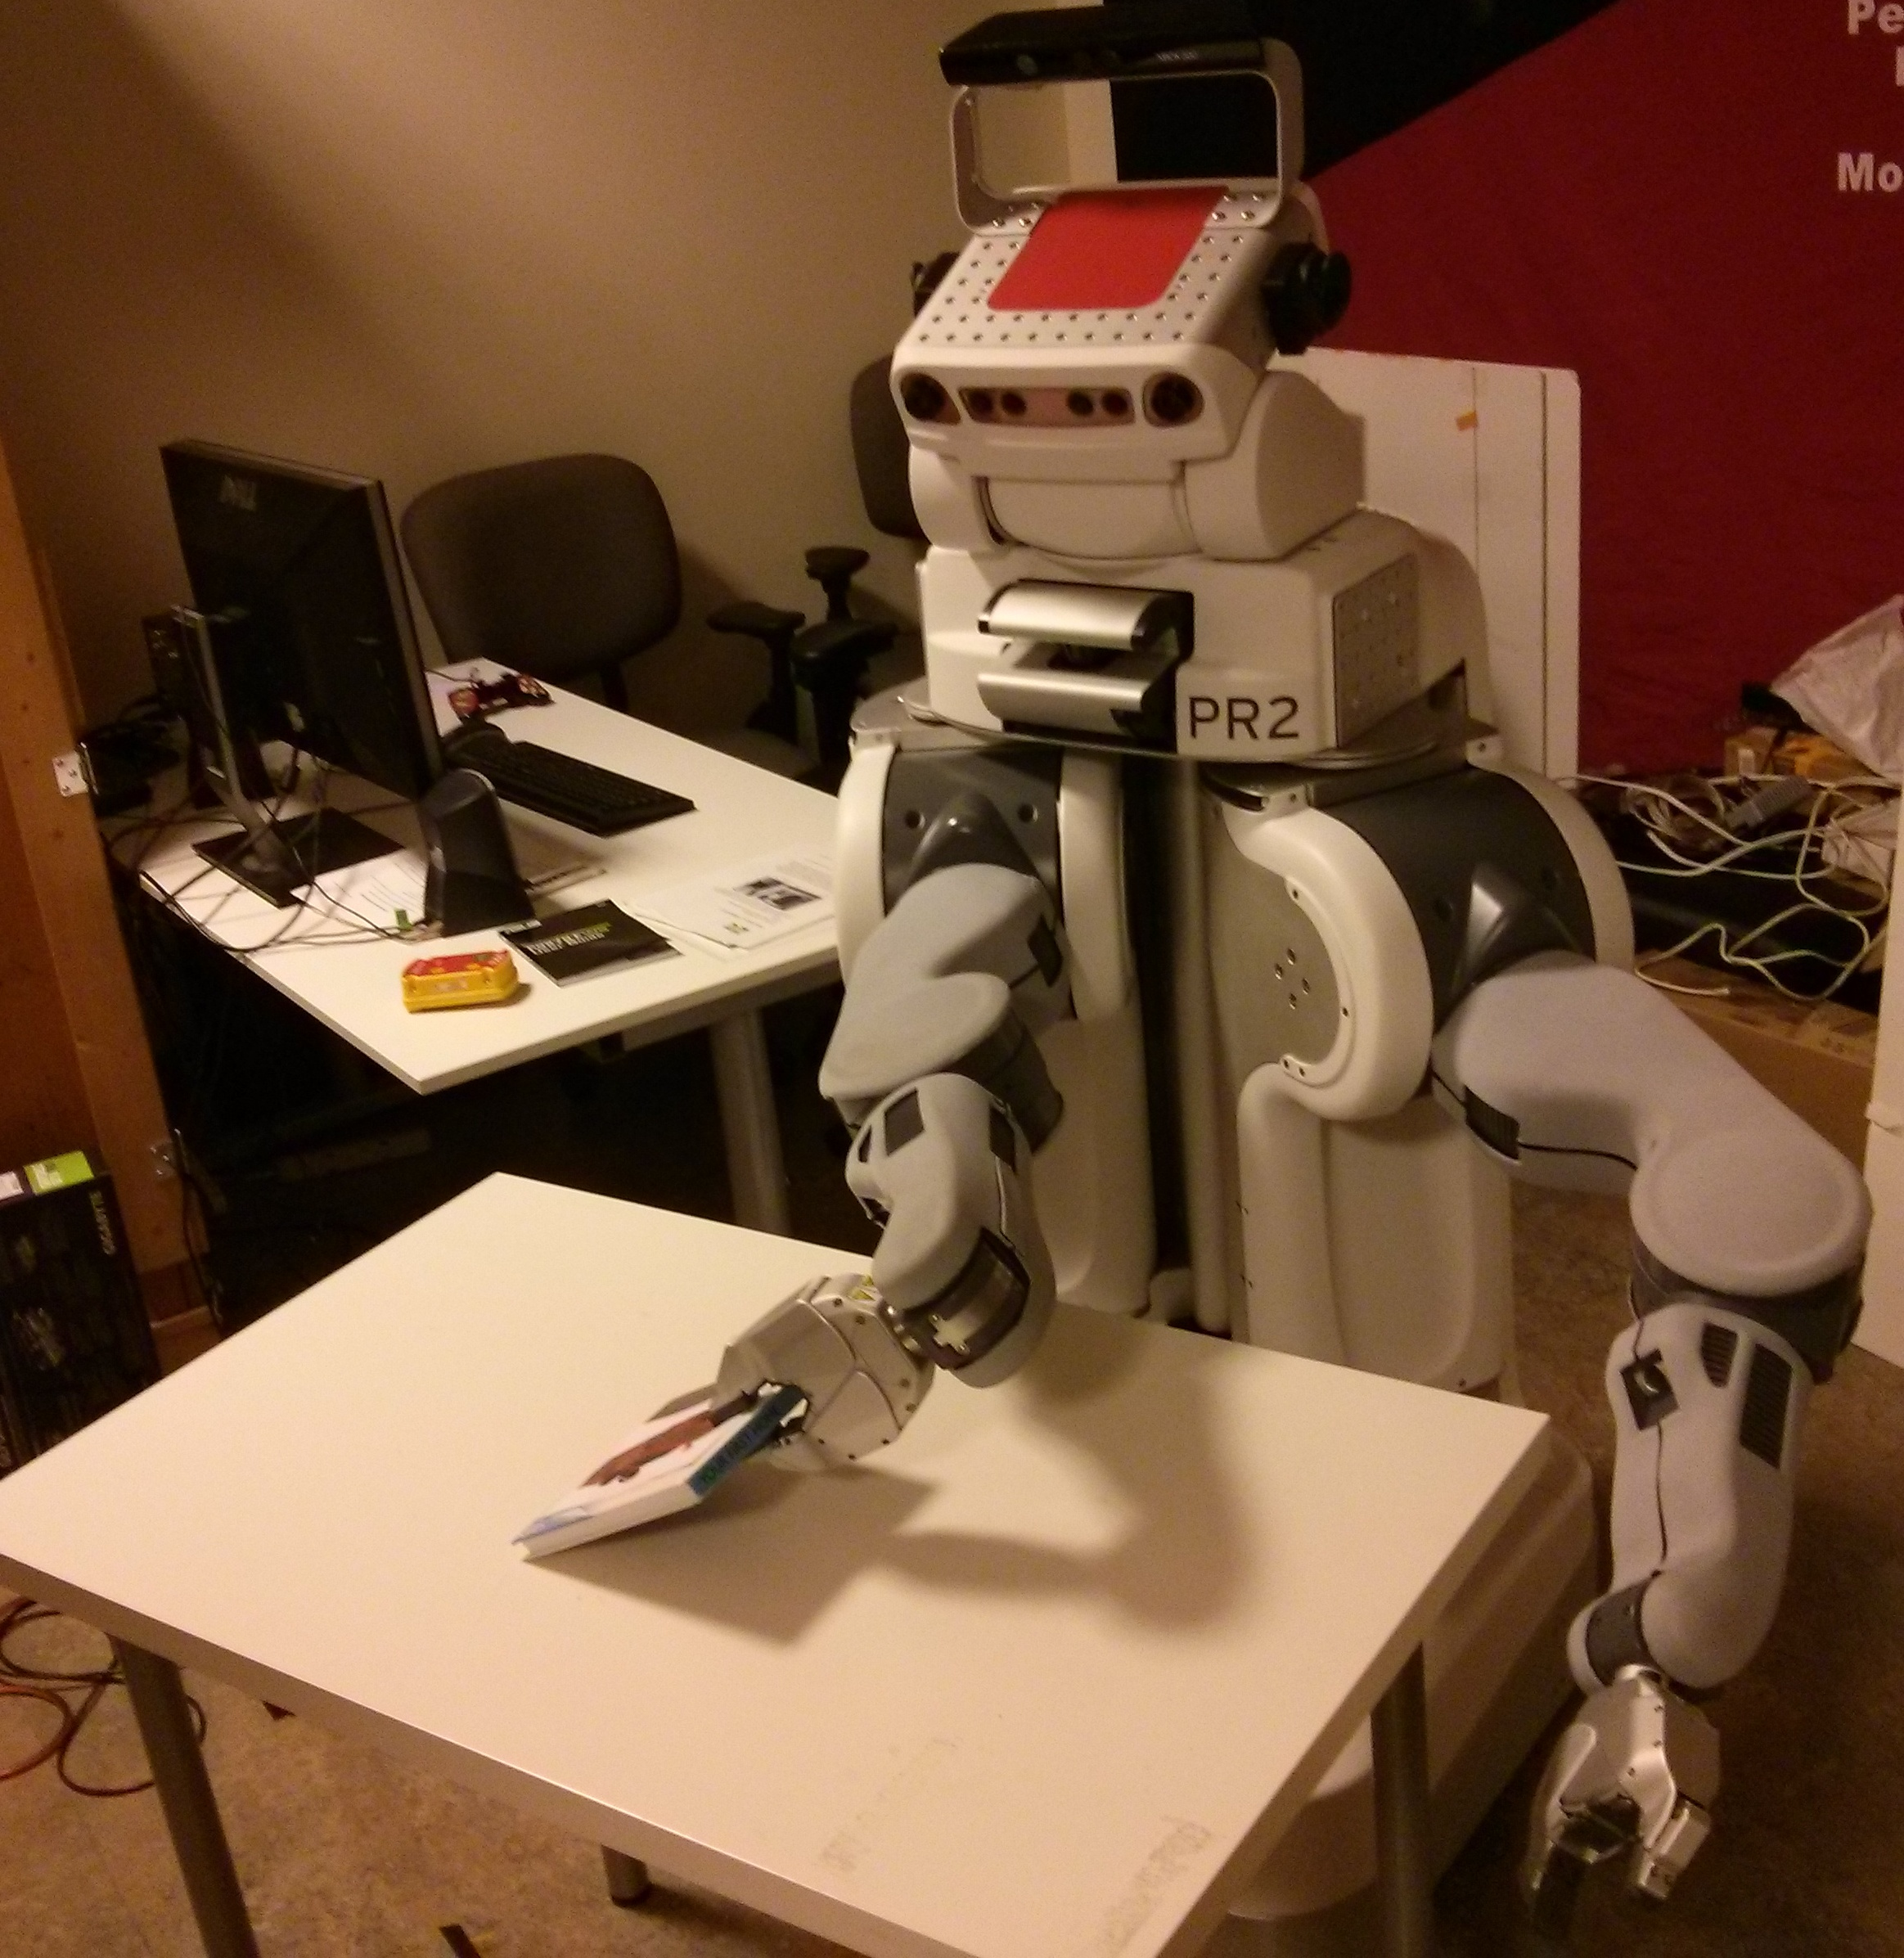
\includegraphics[width=0.45\columnwidth]{pics/pr2_rotate.jpg}}
    \end{tabular}
    \caption{Top-left: The PR2 robot trying to recognize a book based the the back. This pose is ambiguous between book 1 (top-right, NE and NW) and book 2, (top-right, SE and SW). The PR2 takes the optimal action of flipping the book over (bottom-left, bottom-right) in order to confidently predict the identity of the object.}
    \label{fig:pr2}
    \end{figure}

    %contributions
    %* novel probabilistic model for object recognition
    %* action selection probabilistic algorithm to pick the optimal action in order to recognize the object
